\documentclass[tikz,border=2pt]{standalone}
\usepackage{amsmath,amssymb}
\usepackage{pgfplots}
\pgfplotsset{compat=1.18}

\begin{document}
% Y | X = x ~ Pois(x): E[Y | X = x] = x. Given X = x the factor h(x) = x is a known number,
% so E[X Y | X = x] = x * E[Y | X = x] = x^2.
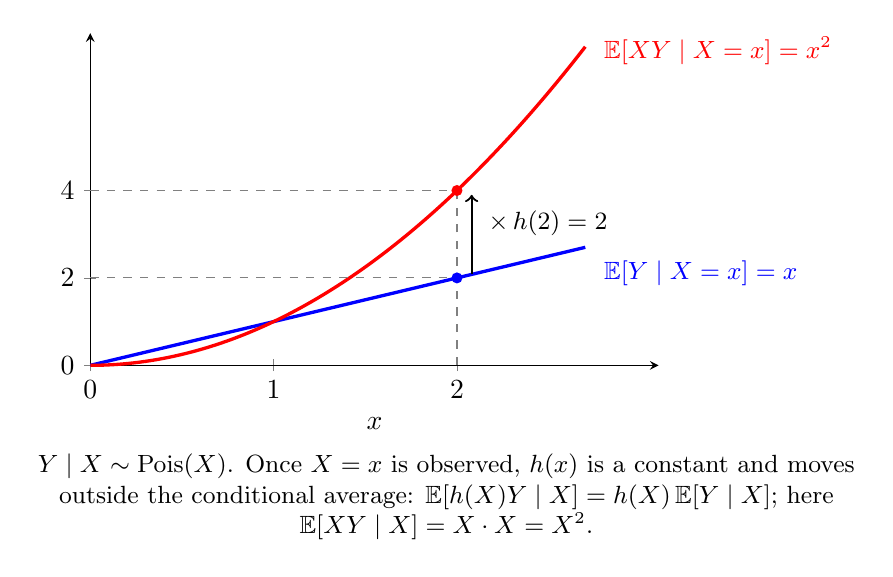
\begin{tikzpicture}
	\begin{axis}[
		axis lines=left, xmin=0, xmax=3.1, ymin=0, ymax=7.6,
		xtick={0,1,2}, ytick={0,2,4},
		xlabel={$x$},
		samples=100, smooth, width=8.8cm, height=5.8cm, clip=false
		]
		\addplot[blue, very thick, domain=0:2.7] {x};
		\addplot[red, very thick, domain=0:2.7] {x^2};
		\draw[gray, dashed] (axis cs:2,0) -- (axis cs:2,4);
		\draw[gray, dashed] (axis cs:0,2) -- (axis cs:2,2);
		\draw[gray, dashed] (axis cs:0,4) -- (axis cs:2,4);
		\fill[blue] (axis cs:2,2) circle (2pt);
		\fill[red] (axis cs:2,4) circle (2pt);
		\draw[->, thick] (axis cs:2.08,2.1) -- (axis cs:2.08,3.9);
		\node[anchor=west, font=\small] at (axis cs:2.12,3.25) {$\times\,h(2)=2$};
		\node[blue, anchor=north west, font=\small] at (axis cs:2.75,2.62) {$\mathbb{E}[Y\mid X=x]=x$};
		\node[red, anchor=west, font=\small] at (axis cs:2.75,7.2) {$\mathbb{E}[XY\mid X=x]=x^2$};
	\end{axis}
	\node[anchor=north, font=\small, align=flush center, text width=10.4cm] at ([yshift=-2pt]current axis.outer south) {$Y\mid X\sim\operatorname{Pois}(X)$. Once $X=x$ is observed, $h(x)$ is a constant and moves outside the conditional average: $\mathbb{E}[h(X)Y\mid X]=h(X)\,\mathbb{E}[Y\mid X]$; here $\mathbb{E}[XY\mid X]=X\cdot X=X^2$.};
\end{tikzpicture}
\end{document}
